%%%%%%%%%%%%%%
%% Run LaTeX on this file several times to get Table of Contents,
%% cross-references, and citations.
%% w-bktmpl.tex. Current Version: Feb 16, 2012
%%%%%%%%%%%%%%%%%%%%%%%%%%%%%%%%%%%%%%%%%%%%%%%%%%%%%%%%%%%%%%%%
%  Template file for
%  Wiley Book Style, Design No.: SD 001B, 7x10
%  Wiley Book Style, Design No.: SD 004B, 6x9
%
%  Prepared by Amy Hendrickson, TeXnology Inc.
%  http://www.texnology.com
%%%%%%%%%%%%%%%%%%%%%%%%%%%%%%%%%%%%%%%%%%%%%%%%%%%%%%%%%%%%%%%%

%%%%%%%%%%%%%%%%%%%%%%%%%%%%%%%%%%%%%%%%%%%%%%%%%%%%%%%%%%%%%%%%
%% Class File
%% For default 7 x 10 trim size:
\documentclass{WileySev}
%% Or, for 6 x 9 trim size
%\documentclass{WileySix}
%%%%%%%%%%%%%%%%%%%%%%%%%%%%%%%%%%%%%%%%%%%%%%%%%%%%%%%%%%%%%%%%
%% Post Script Font File
% For PostScript text
% If you have font problems, you may edit the w-bookps.sty file
% to customize the font names to match those on your system.
\usepackage{w-bookps}
%% Adding hyperlink content to the table of contents
\usepackage{color}   %May be necessary if you want to color links
\usepackage{hyperref}
\hypersetup{
    colorlinks=true, %set true if you want colored links
    linktoc=all,     %set to all if you want both sections and subsections linked
    linkcolor=blue,  %choose some color if you want links to stand out
}
%% Adding MATLAB code, figures and other useful packages 
\definecolor{mypink2}{RGB}{219,48,122}
\definecolor{mygray}{RGB}{100,100,100}
\definecolor{myturq}{RGB}{0,206,209}
\definecolor{mygreen}{RGB}{50,205,50}

\usepackage{listings}
\lstset{
    language=R,
    basicstyle=\scriptsize\ttfamily,
    commentstyle=\ttfamily\color{mygray},
    %numbers=left,
    %numberstyle=\ttfamily\color{blue}\footnotesize,
    stepnumber=1,
    numbersep=5pt,
    backgroundcolor=\color{white},
    showspaces=false,
    showstringspaces=false,
    showtabs=false,
    frame=single,
    tabsize=2,
    captionpos=b,
    breaklines=true,
    breakatwhitespace=false,
    title=\lstname,
    escapeinside={},
    keywordstyle=\bfseries\color{blue},
    morekeywords={myturq}
    }
%\usepackage{mcode}
\usepackage{subcaption}
%%%%%%%
%% For times math: However, this package disables bold math (!)
%% \mathbf{x} will still work, but you will not have bold math
%% in section heads or chapter titles. If you don't use math
%% in those environments, mathptmx might be a good choice.

% \usepackage{mathptmx}

%%%%%%%%%%%%%%%%%%%%%%%%%%%%%%%%%%%%%%%%%%%%%%%%%%%%%%%%%%%%%%%%
%% Graphicx.sty for Including PostScript .eps files
\usepackage{graphicx}

%%%%%%%%%%%%%%%%%%%%%%%%%%%%%%%%%%%%%%%%%%%%%%%%%%%%%%%%%%%%%%%%
%% Other packages you might want to use:

% for chapter bibliography made with BibTeX
\usepackage{chapterbib}
\usepackage{natbib}

% for multiple indices
% \usepackage{multind}

% for answers to problems
% \usepackage{answers}
\usepackage{multirow}
\usepackage{tcolorbox}
\tcbuselibrary{skins}
\newcommand{\myexample}[2]{
    \begin{tcolorbox}[enhanced,colback=black!5!white,colframe=black,sharp corners,title={Example: #1}]#2
    \end{tcolorbox}
}
%%%%%%%%%%%%%%%%%%%%%%%%%%%%%%%%%%%%%%%%%%%%%%%%%%%%%%%%%%%%%%%%
%% Change options here if you want:
%%
%% How many levels of section head would you like numbered?
%% 0= no section numbers, 1= section, 2= subsection, 3= subsubsection
%%==>>
\setcounter{secnumdepth}{3}

%% How many levels of section head would you like to appear in the
%% Table of Contents?
%% 0= chapter titles, 1= section titles, 2= subsection titles, 
%% 3= subsubsection titles.
%%==>>
\setcounter{tocdepth}{2}

%% Cropmarks? good for final page makeup
%% \docropmarks %% turn cropmarks on

%%%%%%%%%%%%%%%%%%%%%%%%%%%%%%%%%%%%%%%%%%%%%%%%%%%%%%%%%%%%%%%%
%% DRAFT
%
% Uncomment to get double spacing between lines, current date and time
% printed at bottom of page.
% \draft
% (If you want to keep tables from becoming double spaced also uncomment
% this):
% \renewcommand{\arraystretch}{0.6}
%%%%%%%%%%%%%%%%%%%%%%%%%%%%%%

\begin{document}

%%%%%%%%%%%%%%%%%%%%%%%%%%%%%%%%%%%%%%%%%%%%%%%%%%%%%%%%%%%%%%%%
%% Title Pages
%%
%% Wiley will provide title and copyright page, but you can make
%% your own titlepages if you'd like anyway

%% Setting up title pages, type in the appropriate names here:
\booktitle{Experimental Design and Statistical Analysis}
\subtitle{}

\author{William Cruz}%\affil{National Cheng Kung University - Taiwan}
%or
%\authors{}
%% \\ will start a new line.
%% You may add \affil{} for affiliation, ie,
%\authors{Robert M. Groves\\
%\affil{Universitat de les Illes Balears}
%Floyd J. Fowler, Jr.\\
%\affil{University of New Mexico}
%}

%% Print Half Title and Title Page:
%\halftitlepage
\titlepage
%%%%%%%%%%%%%%%%%%%%%%%%%%%%%%%%%%%%%%%%%%%%%%%%%%%%%%%%%%%%%%%%
%% Off Print Info

%% Add your info here:
\offprintinfo{Experimental Design and Statistical Analyses \\ First edition}{William Cruz}
%% Can use \\ if title, and edition are too wide, ie,
%% \offprintinfo{Survey Methodology,\\ Second Edition}{Robert M. Groves}
%%%%%%%%%%%%%%%%%%%%%%%%%%%%%%%%%%%%%%%%%%%%%%%%%%%%%%%%%%%%%%%%
%% Copyright Page

\begin{copyrightpage}{2019}
Experimental Design and Statistical Analyses
\end{copyrightpage}

% Note, you must use \ to start indented lines, ie,
% 
% \begin{copyrightpage}{2004}
% Survey Methodology / Robert M. Groves . . . [et al.].
% \       p. cm.---(Wiley series in survey methodology)
% \    ``Wiley-Interscience."
% \    Includes bibliographical references and index.
% \    ISBN 0-471-48348-6 (pbk.)
% \    1. Surveys---Methodology.  2. Social 
% \  sciences---Research---Statistical methods.  I. Groves, Robert M.  II. %
% Series.\\

% HA31.2.S873 2004
% 001.4'33---dc22                                             2004044064
% \end{copyrightpage}

%%%%%%%%%%%%%%%%%%%%%%%%%%%%%%%%%%%%%%%%%%%%%%%%%%%%%%%%%%%%%%%%
%% Frontmatter >>>>>>>>>>>>>>>>

%%%%%%%%%%%%%%%%%%%%%%%%%%%%%%%%%%%%%%%%%%%%%%%%%%%%%%%%%%%%%%%%
%% Only Dedication (optional) 
%% or Contributor Page for edited books
%% before \tableofcontents
\dedication{To my family}
% ie,
%\dedication{To my parents}
%%%%%%%%%%%%%%%%%%%%%%%%%%%%%%%%%%%%%%%%%%%%%%%%%%%%%%%%%%%%%%%%
%  Contributors Page for Edited Book
%%%%%%%%%%%%%%%%%%%%%%%%%%%%%%%%%%%%%%%%%%%%%%%%%%%%%%%%%%%%%%%%

% If your book has chapters written by different authors,
% you'll need a Contributors page.

% Use \begin{contributors}...\end{contributors} and
% then enter each author with the \name{} command, followed
% by the affiliation information.

% \begin{contributors}
% \name{Masayki Abe,} Fujitsu Laboratories Ltd., Fujitsu Limited, Atsugi,
% Japan

% \name{L. A. Akers,} Center for Solid State Electronics Research, Arizona
% State University, Tempe, Arizona

% \name{G. H. Bernstein,} Department of Electrical and
% Computer Engineering, University of Notre Dame, Notre Dame, South Bend, 
% Indiana; formerly of
% Center for Solid State Electronics Research, Arizona
% State University, Tempe, Arizona 
% \end{contributors}

%%%%%%%%%%%%%%%%%%%%%%%%%%%%%%%%%%%%%%%%%%%%%%%%%%%%%%%%%%%%%%%%
\contentsinbrief %optional
\tableofcontents
\listoffigures %optional
\listoftables  %optional

%%%%%%%%%%%%%%%%%%%%%%%%%%%%%%%%%%%%%%%%%%%%%%%%%%%%%%%%%%%%%%%%
% Optional Foreword:

%\begin{foreword}
%text
%\end{foreword}

%%%%%%%%%%%%%%%%%%%%%%%%%%%%%%%%%%%%%%%%%%%%%%%%%%%%%%%%%%%%%%%%
% Optional Preface:

%\begin{preface}
% text
%\prefaceauthor{}
%\where{place\\
% date}
%\end{preface}

% ie,
% \begin{preface}
% This is an example preface.
% \prefaceauthor{R. K. Watts}
% \where{Durham, North Carolina\\
% September, 2004}

%%%%%%%%%%%%%%%%%%%%%%%%%%%%%%%%%%%%%%%%%%%%%%%%%%%%%%%%%%%%%%%%
% Optional Acknowledgments:

% \acknowledgments
% acknowledgment text
% \authorinitials{} % ie, I. R. S.


%%%%%%%%%%%%%%%%%%%%%%%%%%%%%%%%
%% Glossary Type of Environment:

% \begin{glossary}
% \term{<term>}{<description>}
% \end{glossary}

%%%%%%%%%%%%%%%%%%%%%%%%%%%%%%%%
\begin{acronyms} 
\acro{LMM}{Linear Mixed Model}
\acro{BIB}{Balanced Incomplete Block}
\end{acronyms}

%%%%%%%%%%%%%%%%%%%%%%%%%%%%%%%%
%% In symbols environment <term> is expected to be in math mode; 
%% if not in math mode, use \term{\hbox{<term>}}

% \begin{symbols}
% \term{<math term>}{<description>}
% \term{\hbox{<non math term>}}Box used when not using a math symbol.
% \end{symbols}

%%%%%%%%%%%%%%%%%%%%%%%%%%%%%%%%
\begin{glossary}
\term{mean}{Average among observations}
\end{glossary}
%%%%%%%%%%%%%%%%%%%%%%%%%%%%%%%%%%%%%%%%%%%%%%%%%%%%%%%%%%%%%%%%
\begin{introduction}
Experimental Design is at the core of research

\end{introduction}

%%%%%%%%%%%%%%%%%%%%%%%%
%% Optional Part : 1 %%%
%%%%%%%%%%%%%%%%%%%%%%%%
\part[1 Experimental Design]
{The Experimental Design}

\chapter[The Experimental Design]
{The Experimental Design}

\section{Basics of Experimental Design}

As defined by Leedy, research is a systematic quest for undiscovered truth \cite{leedy2005practical}. In this definition, the quest is systematic because it uses scientific procedures to solving a problem and the truth sought, should be something that is unknown at the time, which implies that the researcher has conducted a thoughtful literature search to ascertain that the answer to the experimental question was not addressed in previous studies.

A \textit{true experiment} may be defined as a study in which certain independent variables are manipulated, their effect on one or more dependent variables is determined, and the levels (i.e. values) of these independent variables are assigned at random to the experimental units in the study. Such experiments allow the researcher to develop a statistical model and estimate its validity. An \textit{experimental unit} must be carefully defined; it may be a part, a person, a class, a month, or some other unit depending of the problem. The experimental units make up a \textit{universe} of all such units, present or future, and a \textit{population} is defined as measurements that might be taken on all experimental units in the universe. There may be several populations defined on the same experimental units \cite{hicks1999fundamental}.

Manipulation and randomization are essential for a true experiment from which one may be able to infer cause and effect. Sometimes it is not always feasible to assign some variables to the experimental units at random; although it may be possible to assign some variables to the experimental units at random, it may be possible to run a \textit{quasi-experiment} in which groups of units are assigned to various levels of the independent variable randomly. Randomizing is a technique used to assure a high probability of group equality on many variables that escape of proper control.

There are other types of research that are not experimental. One of the most common is the \textit{ex-post-facto} research. The values of the variables have been determined by circumstances beyond the control of the experimenter, the variables have already acted, and the research measure only what has occurred (e.g. Studies showing a high incidence of cancer in people who smoke heavily). However, such inferences are dangerous, since the researches cannot claim causality unless they are able to rule out other competing hypotheses. In this category are survey research, historical research and developmental research. All these investigations may use statistical methods to analyze data collected but none is really experimental in nature. There are three phases to bear in mind to make a meaningful study: The planning stage, the design stage and the analysis.
\\
\myexample{Experimental Designs}{Illustrations of true experiments and ex-post-facto experiments often use techniques such as regression and correlation. For example in a regression problem, levels of the independent variable $X$ are set, a level of $X$ is assigned at random to each experimental unit, observations are made on the dependent variable $Y$, and an equation for predicting $Y$ from $X$ over the range of specified $X's$ is sought. Such studies are true experiments.
A correlation problem may involve a sample of experimental units for which two variables ($X$ and $Y$) have acted, the resulting ($x$ and $y$) pairs are plotted to look for a relationship, and a correlation coefficient is calculated to measure the strength of the relationship. Such studies are ex-post-facto studies.}

\section{The Experiment}

The experiment includes a statement of the problem to be solved. A careful statement of the problem goes a long way toward its solution. Much care must be taken to spell out the problem in terms that are well understood and point the way in which the research might be conducted.

\subsection{Response variables}

The statement of the problem must include reference to a least one characteristic of an experimental unit on which information is to be obtained. Such characteristics are called \textit{response} or 
\textit{dependent variables}. The response variable may be \textit{qualitative} or \textit{quantitative} response. The outcome of a true experiment occurs at random, so a response variables is a random variable. Knowledge of such a variable is essential because the shape of its distribution often dictates what statistical test can be used in subsequent data analysis. In addition to a statement of the problem that includes reference to a response variable, one must ask the following questions about the measurement method.

\begin{itemize}
\item
What instruments are necessary to measure the variable?
\item
How accurately can the variable be measured?
\end{itemize}

\subsection{Independent variables}

Many controllable experimental variables, called independent variables or factors, may contribute to the value of the response variable. \textit{Qualitative factors} have levels that vary by category rather than numerical degree. \textit{Quantitative factors},  have levels that are counts of measurements. The experimenter must decide which factors will be held constant, to be manipulated at certain specified levels, and which will be averaged out by a process of randomization.

Factors whose levels are set at specified values are called \textit{fixed effects}, and those whose levels are randomly selected from all possible levels are called \textit{random effects}. When at least two factors are being considered, one must also ask: How are the factor levels to be combined? Each combination of levels from two or more factors is called a \textit{treatment combination}. If at least one value of the response is observed at each treatment combination, the experiment is called a (complete) \textit{factorial experiment}, as in Table \ref{tab:factorial_array}. An experiment in which the levels of one factor are chosen within the levels of another factor is a \textit{nested experiment}, as in Table \ref{tab:nested_array}.
\\
\myexample{Factorial Experiment}{Consider an experiment in which the factor $A$ is to be considered at three levels, and a second factor $B$ is to be considered at two levels. Two observations are to be made at each treatment combination. If the $3 \times 2 = 6$ treatment combinations can be set in the following way, a factorial experiment will be possible. Notice that both levels of factor $B$ can be used with the three levels of factor $A$.}

\begin{table}[h]
\caption{Factorial Experiment Arrangement}
\centering
\begin{tabular}{ c|ccc }
\hline
\multicolumn{4}{c}{\textbf{Factor A}} \\
\hline
\textbf{Factor B} & 1 & 2 & 3 \\
\hline
\multirow{3}{6em}{1} & --- & --- & --- \\
& --- & --- & --- \\
& --- & --- & --- \\
\hline
\multirow{3}{6em}{2} & --- & --- & --- \\
& --- & --- & --- \\
& --- & --- & --- \\
\hline
\end{tabular}
\label{tab:factorial_array}
\end{table}

\myexample{Nested Experiment}{Sometimes one chooses three suppliers and randomly selects two batches of material from each for chemical analysis, letting $A$ denote the supplier and $B$ denote the batch. Such an experiment has the nested arrangement, as illustrated in Table ~\ref{tab:nested_array}. This involves six sets of data, like the factorial arrangement in Table ~\ref{tab:factorial_array}, but now the factors are in a decidedly different arrangement. The two levels of factor $B$ associated with level 1 of factor $A$ cannot be used with levels 2 and 3 of factor $A$.}

\begin{table}[h]
\caption{Nested Experiment Arrangement}
\centering
\begin{tabular}{ cccccc }
\hline
\multicolumn{6}{c}{\textbf{Supplier $A$}} \\
\multicolumn{2}{c}{1} & \multicolumn{2}{c}{2} & \multicolumn{2}{c}{3} \\
\hline
\multicolumn{2}{c}{\textbf{Batch $B$}} & \multicolumn{2}{c}{\textbf{Batch $B$}} & \multicolumn{2}{c}{\textbf{Batch $B$}} \\
1 & 2 & 3 & 4 & 5 & 6 \\
\hline
--- & --- & --- & --- & --- & --- \\
--- & --- & --- & --- & --- & --- \\
--- & --- & --- & --- & --- & --- \\
\hline
\end{tabular}
\label{tab:nested_array}
\end{table}

\section{The Design}

The investigator needs an experimental design for obtaining data that provide objective results with a minimum expenditure of time and resources. In order to correctly assess how many observations are needed, one have to considerate three aspects: how large a difference is to be detected, how much variation is present, and what size risks can be tolerated. If such information is missing, one best advised to take as large a sample as possible. In practice, the sample size is often quite arbitrary; however, the availability of tables and statistical software often make it possible to determine the sample size in an objective fashion \cite{hicks1999fundamental}.
% pending to expand examples on how to determine sample size

Once a decision has been made to control certain variables at specified levels, there are always a number of other variables that cannot be controlled. To average out the effects of these uncontrolled variables, it is necessary to randomize the order of experimentation. Randomization will allow the experimenter to assume that the measurement errors are independent, a common assumption in most statistical analyses. Independent variables may be purposefully introduced into the study because they are of interest, because they represent restrictions on randomization, or, indeed, because they are somewhat extraneous and not of interest to the experimenter. When deciding how such variables should be handled, one should seek to maximize the systematic variation of factors of interest and to minimize error (i.e. unexplained) variation, including so-called errors of measurement, by controlling the systematic variation of the factors that are not of interest. Kerlinger refers to this as the max-min-con principle of experimental design. Are basically three ways to handle independent variables:

\begin{itemize}
\item
Rigid control, the factors remain fixed throughout the experiment
\item
Manipulate or set at levels of interest.
\item
Randomization
\end{itemize}

When factors remain fixed, any inferences drawn from the experiment are valid only for the fixed conditions. Variables that are manipulated or set at levels of interest are those whose effects on the response variable are to be studied. They may be either qualitative or quantitative, and their levels may be either fixed or random. Every effort should be made to include extreme levels, to provide the opportunity to maximize any effects that may be present. 

On a different account, it is also of prime importance that the order of experimentation\footnote{This means that each observation within an experiment is taken in a random order after tossing a dice or flipping a coin} is randomized in order to average out the effects of variables that cannot be controlled, such as indicated by the numbers in Table~\ref{tab:rando_factorial}; such averaging does not remove those effects completely, they only increase the variation in the observed data.

\begin{table}[h]
\caption{Randomization in a Factorial Experiment}
\centering
\begin{tabular}{ c|ccc }
\hline
\multicolumn{4}{c}{\textbf{Factor A}} \\
\hline
\textbf{Factor B} & 1 & 2 & 3 \\
\hline
\multirow{3}{6em}{1} & 10 & 18 & 6 \\
& 11 & 5 & 1 \\
& 17 & 16 & 2 \\
\hline
\multirow{3}{6em}{2} & 9 & 3 & 14 \\
& 4 & 7 & 15 \\
& 12 & 8 & 13 \\
\hline
\end{tabular}
\label{tab:rando_factorial}
\end{table}

Once the experimenters have agreed upon the experimental design and the randomization procedure, they can set up a mathematical model to describe the experiment. This model will show the response variable as a function of all factors to be studied and any restrictions imposed on the experiment as a result of the method of randomization. A typical model description for the experiment layout presented in Table~\ref{tab:rando_factorial} is as described in Equation \ref{eq:1}

\begin{equation}
Y_{ij}= \mu+\beta_i+\tau_j+\varepsilon_{(ij)} \label{eq:1} % Basis equation
\end{equation}
\\
with $Y_{ij}$  the measured variable, $\mu$ a common effect in all observations, $\beta_i$ the \textbf{Factor B} effect (where $i = 1, 2$), and $\tau_j$ the \textbf{Factor A} effect (where $j = 1, 2, 3$), and $\varepsilon_{(ij)}$ the random error in the experiment.

Finally and since the objective of the research is to shed light on a stated problem, one next expresses the problem in terms of a testable \textit{hypotheses}. A research hypothesis is a formal statement of what the experimenter expects to find in the data. For example, the $i$ treatments will produce different averages of the response variable. Statisticians usually state their hypotheses in null form, since these are the only easily testable statements. For example, the $i$ treatments average will not have significant differences. A null hypothesis usually can be expressed in terms of the mathematical model set up in the last step of the design phase.

\section{The Analysis}

This step starts with data collection as described in connection with the design. If the experiment is complicated, a pilot run may be used to check details and make sure that no critical details have been overlooked. Once collected, the data should be prepared for manual or computer analysis. The preparation of graphical displays, inspection of those displays, and computation of appropriate numerical summaries follows data collection. The decisions about what analyses to perform should be expressed in terms that are meaningful for both, to the experimenter and to those expected to receive the report.
An investigative process has built-in self-correction. It is an iterative process that moves us closer to the truth at each stage. Statistics enters such process at two points: (1) the design of the experiment and (2) the analysis and interpretation of the experimental results. When certain hypotheses appear to be tenable, these results should be used as feedback to design a better experiment.

\section{Examples}

Examples 1.5.1 and 1.5.2 from \cite{hicks1999fundamental} are but two illustrations of how projects are organized into three phases: experiment, design and analysis.

\subsection{Salk Vaccine Experiment}

The mathematical model of this experiment could be written as

\begin{equation}
Y_{ij}= \mu+\tau_j+\varepsilon_{ij} \label{eq:2} % Basis equation
\end{equation}
\\
Where $Y_{ij}$ is equal to 0 or 1: 0 if no polio is diagnosed and 1 if polio is found. The subscript
$i$ represents the child, a number from 1 to approximately 200000. The subscript $j$ represents the treatment received by the $i^{th}$ child: 1 if treated with Salk vaccine and 2 if treated with a placebo. $\mu$ is a constant or general average of the 0's and 1's for the whole population, $\tau_j$ is the effect of the $j^{th}$ treatment, and $\varepsilon_{ij}$ is a random error associated with the $i^{th}$ child receiving treatment $j$.

 Letting $n_j$ denote the number of children who receive treatment $j$, the proportion of children contracting polio who received treatment $j$ is

 \begin{equation}
P_j=\frac{\sum_{i=1}^{n_j} Y_{ij}}{n_j}\label{eq:3}
 \end{equation}
\\
and the proportion contracting polio in the total sample of $n=n_1+n_2$ children is 

\begin{equation}
P=\frac{\sum_{i=1}^{n_1} Y_{i1} + \sum_{i=1}^{n_2} Y_{i2}}{n_1 + n_2}\label{eq:4}
\end{equation}
\\
Use of $P_j$ indicates that the proportion contracting polio who receive treatment $j$ is a random variable \textit{before} the experiment is conducted. The observed proportion  \textit{after} conducting the experiment is denoted $p_j$.
Letting $\theta_j$ denote the true proportion in the $j^{th}$ population who contract polio, the statistical hypothesis to be tested is

\begin{equation}
H_0=\theta_1=\theta_2
\end{equation}
\\
with alternative
\begin{equation}
H_0=\theta_1<\theta_2
\end{equation}
\\
The form of the alternative hypothesis indicates that we are interested in showing that the true proportion contracting polio will be less for treatment 1 (\textit{vaccine}) than for treatment 2 (\textit{placebo}).
Approximately $0.09\%$ of all children contract polio, and (200,000)(0.0009)=180 is sufficiently large, so the sample proportions have approximately normal distribution. Thus,

\begin{equation}
Z=\frac{P_1+P_2}{\sqrt{P(1-P)[(1/n_1)+(1/n_2)]}}\label{eq:5}
\end{equation}
\\
is an appropriate test statistic. When the null hypothesis ($H_0=\theta_1=\theta_2$) is true, $Z$ has an approximate normal distribution with mean 0 and variance 1.
The results of the experiment are summarized in Table ~\ref{tab:polio}. When Equations ~\ref{eq:3}, ~\ref{eq:4} and ~\ref{eq:5} are used with those results, an observed value of

\begin{equation}
z\approx \frac{(28\times10^{-5})-(71\times10^{-5})}{\sqrt{[49\times10^{-5}][1-(49\times10^{-5})][(1/200,745)+(1/201,229)]}}\approx-6.14
\end{equation}
\\
is obtained. The probability of observing a value of $Z$ as extreme as $-6.14$ when the null hypothesis is true is $P(Z\leq-6.14)\approx4.126\times10^{-10}$. Thus, the likelihood of observing a difference of this magnitude when the Salk vaccine has no effect is less than one in a billion. This gives a very strong indication that the researchers should reject $H_0$ and conclude that the vaccine is effective. Conversely the R code for obtaining this result can be found below.

\begin{table}[h]
\caption{Polio Experiment Results}
\centering
\begin{tabular}{ cccc }
\hline
\textbf{Treatment} & \textbf{Sample Size} & \textbf{Number Contracting Polio} & \textbf{Proportion Contracting Polio} \\
\hline
\textit{Salk Vaccine} & $n_1=200,745$ & 56 & $p_1\approx 28\times 10^{-5}$ \\
\textit{Placebo} & $n_2=201,229$ & 142 & $p_2\approx 71\times 10^{-5}$ \\
\hline
\textit{Totals} & $n=401,974$ & 198 & $p\approx 49\times 10^{-5}$ \\
\hline
\end{tabular}
\label{tab:polio}
\end{table}

\begin{lstlisting}[language=R]
n1 <- 200745      # sample size of those who received Salk vaccine as treatment
n2 <- 201229      # sample size of those who received placebo as treatment
n  <- n1 + n2     # Total sample size
num_pol1 <- 56    # Number of children who contracted polio and received Salk vaccine
num_pol2 <- 142   # Number of children who contracted polio and received Placebo
num_pol  <- num_pol1+num_pol2 # Total number of children who contracted polio
P1 <- num_pol1/n1 # Proportion of children who were diagnosed with polio and received Salk vaccine 1-((n1-num_pol1)/n1)
P2 <- num_pol2/n2 # Proportion of children who were diagnosed with polio and received Placebo      1-((n2-num_pol2)/n2)
P  <- num_pol/n   
z  <- (P1 - P2)/sqrt((P*(1-P))*((1/n1)+(1/n2)))
\end{lstlisting}

\subsection{Cutting Tool Experiment}

An experiment was to be designed to study the effect of several factors on the power requirements for cutting metal with ceramic tools. The metal was cut on a lathe, and the vertical component of a dynamometer reading. Since this component is proportional to the horsepower requirements in making the cut, it was taken as the measured variable, $Y$. The vertical component is measured in millimeters of deflection on a recording instrument. Some of the factors that might affect this deflection are tool types, angle of tool edge bevel, type of cut, depth of cut, feed rate, and spindle speed. It was agreed to hold some factors constant because they represent typical operating conditions. The main objective of the study was to determine the effect of three factors (tool type, angle of edge bevel, and type of cut) on the power requirements. Since only two ceramic tool types were available, this factor was considered at two levels. The angle of tool edge bevel was also set at two levels. 15º and 30º, representing the extremes for normal operation. The type of cut was either continuous or interrupted, two levels.

There are therefore two fixed levels for each of three factors or $2^3$ conditions, this is called a $2^3$ factorial experiment. The levels of two factors (type of tool and type of cut) are qualitative, whereas the angle of edge bevel is a quantitative factor. It was decided to take four observations under each of the eight conditions, making a total of 32 runs in a completely randomized order. Complete randomization ensures the averaging out of any effects that might be correlated with the time of the experiment. The mathematical model for this experiment and design would be

\begin{equation}
Y_{ijkm}=\mu+T_i+B_j+TB_{ij}+C_k+TC_{ik}+BC_{jk}+TBC_{ijk}+E_{m(ijk)}
\end{equation}
\\
with $Y_{ijkm}$ the measured variable, $\mu$ a common effect in all observations (the true mean of the population from which all the data came), $T_i$ the tool type effect (where $i = 1, 2$), $B_j$ the angle of bevel (where $j = 1, 2$) with level 1 the 15º angle, $C_k$ the type of cut (where $k = 1, 2$) with level 1 the continuous cut, and $\varepsilon_{m(ijk)}$ the random error in the experiment (where $m = 1, 2, 3, 4$). The other terms stand for interactions between the main factors $T$, $B$, and $C$. The results in millimeter deflection are given in Table ~\ref{tab:cut_tool}, below it can also be found the R code for generating this data frame and using the package $EMSaov$ with the given model and fixed effects produces the ANOVA summary in Table ~\ref{tab:anova_cut_tool}.
\\
\\
\\
\begin{table}[h]
\caption{Power Requirement Data}
\centering
\begin{tabular}{ |c|cccc| }
\hline
\multirow{4}{*}{Type of Cut, $C$} & \multicolumn{4}{c|}{Tool Type, $T$} \\
%\cline{2-5}
 & \multicolumn{2}{c}{1} & \multicolumn{2}{c|}{2} \\
 \cline{2-5}
 & \multicolumn{2}{c}{Bevel Angle, $B$} & \multicolumn{2}{c|}{Bevel Angle, $B$} \\
 %\cline{2-5}
 & $15^{\circ}$ & $30^{\circ}$ & $15^{\circ}$ & $30^{\circ}$ \\
 \hline
 \multirow{4}{*}{\textit{Continuous}} & 29.0 & 28.5 & 28.0 & 29.5 \\
 & 26.5 & 28.5 & 28.5 & 32.0 \\
 & 30.5 & 30.0 & 28.0 & 29.0 \\
 & 27.0 & 32.5 & 25.0 & 28.0 \\
\hline
\multirow{4}{*}{\textit{Interrupted}} & 28.0 & 27.0 & 24.5 & 27.5 \\
 & 25.0 & 29.0 & 25.0 & 28.0 \\
 & 26.5 & 27.5 & 28.0 & 27.0 \\
 & 26.5 & 27.5 & 26.0 & 26.0 \\
\hline
\end{tabular}
\label{tab:cut_tool}
\end{table}

\begin{table}
\caption{ANOVA for Power Requirement Data}
\centering
\begin{tabular}{|c|c|c|c|c|cc|}
\hline
Source    &      Df&   SS     &     MS   & F value & P value & Sig \\
\hline
tool      &      1 & 2.8203125& 2.8203125&  1.2667 &0.2715   &     \\            
bevel     &      1 &20.3203125&20.3203125&  9.1263 &0.0059   &**   \\     
tool:bevel&      1 & 0.1953125& 0.1953125&  0.0877 &0.7696   &     \\ 
cut       &      1 &31.0078125&31.0078125& 13.9263 &0.001    &**   \\ 
tool:cut  &      1 & 0.0078125& 0.0078125&  0.0035 &0.9533   &     \\  
bevel:cut &      1 & 0.9453125& 0.9453125&  0.4246 &0.5209   &     \\ 
tool:bevel:cut & 1 & 0.1953125& 0.1953125&  0.0877 &0.7696   &     \\
Residuals      & 24&53.4375000& 2.2265625&         &         &     \\     
\hline
Totals         & 31&108.9297  &          &         &         &     \\
\hline
\end{tabular}
\label{tab:anova_cut_tool}
\end{table} 
%\footnotesize{*  Statistically significant with an $\alpha \geq 0.05$}
%\footnotesize{** Statistically significant with an $\alpha \geq 0.01$}
\
\begin{lstlisting}[language=R]
# Power Requirement Data Frame
library(EMSaov) # Required library
power_cut <- structure(list(cut = structure(c(rep(2L,16),c(rep(1L,16))),
                                            .Label = c("Continuous","Interrupted"),
                                            class = "factor"),
                            tool   = structure(c(rep(c(rep(2L,8),rep(1L,8)),2)),
                                               .Label = c("Tool1","Tool2"),
                                               class = "factor"),
                            bevel = structure(c(rep(c(rep(2L,4),rep(1L,4)),4)),
                                              .Label = c("15","30"),
                                              class = "factor"),
                            mil_def = as.numeric(c(27.5, 28, 27, 26, 24.5, 25, 28,
                                                   26, 27, 29, 27.5, 27.5, 28, 25,
                                                   26.5, 26.5, 29.5, 32, 29, 28, 28,
                                                   28.5, 28, 25, 28.5, 28.5, 30,
                                                   32.5, 29, 26.5, 30.5, 27))),
                       .Names = c("cut","tool","bevel","mil_del"),
                       class = "data.frame",
                       row.names = c(NA, -32L))
                       # Analysis of Variance (ANOVA)
Anova_T <- EMSanova(mil_del~tool*bevel*cut,data=power_cut,
                    type=c("F","F","F"),nested=c(NA,NA,NA))
\end{lstlisting}

\begin{figure}
  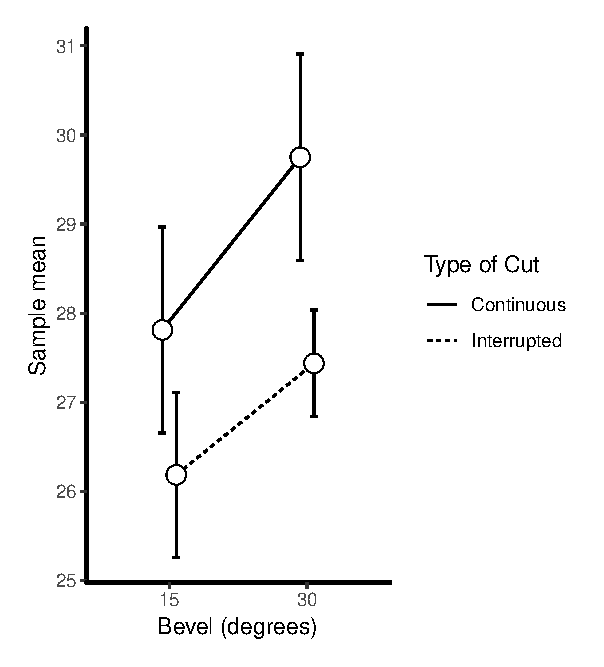
\includegraphics[width=0.5\linewidth]{Ch1_interaction_plot.eps}
  \centering
  \caption{$B \times C$ interaction for power requirement example}
  \label{fig:ch1_interaction}
\end{figure}

\begin{lstlisting}[language=R]
# Interaction plot between factor B and C
library(ggplot2,plyr) # Required libraries
desc_power <- ddply(power_cut,.(cut,bevel),summarise,pw_mean = mean(mil_del),
                    pw_ci = 1.96*sd(mil_del)/sqrt(length(mil_del)))
pd <- position_dodge(width = 0.2)
(ansPlot <-  ggplot(data = desc_power,aes(x=bevel,y=pw_mean,group = cut))+
    geom_line(aes(linetype = cut), position = pd) +
    geom_errorbar(aes(ymin= pw_mean - pw_ci, ymax= pw_mean + pw_ci),
                  width = .1,position = pd, linetype = 1) +
    geom_point(size = 4, position = pd) +
    geom_point(size = 3, position = pd, color = "white") +
    guides(linetype = guide_legend("Type of Cut")) +
    labs(title = c(),x = c("Bevel (degrees)"),
         y = c("Sample mean")) +
    theme(
      panel.background = element_rect(fill = "white"),
      legend.key = element_rect(fill = "white"),
      axis.line.x = element_line(colour = "black", size = 1),
      axis.line.y = element_line(colour = "black", size = 1)
    )
)
\end{lstlisting}

\section{Summary}

\begin{enumerate}
	\item Experiment
	\begin{enumerate}
	\item Statement of problem
    \item Choice of response (dependent) variable
    \item Selection of factors (independent variables) to be varied
    \item Choice of levels of these factors
    	\begin{enumerate}
    		\item Quantitative or Qualitative
		    \item Fixed or random
		\end{enumerate}
	\end{enumerate}
	\item Design
	\begin{enumerate}
		\item Number of observations to be taken
		\item Order of experimentation
		\item Method of randomization to be used
		\item Mathematical model to describe the experiment
		\item Hypotheses to be tested
	\end{enumerate}
	\item Analysis
	\begin{enumerate}
		\item Data collection and processing
		\item Computation of test statistics and preparation of graphics
		\item Interpretation of results for the experimenter
	\end{enumerate}
\end{enumerate}

%\section{Problems}


\chapter[Statistical Inference]{Statistical Inference}

\section{Introduction}

In any experiment, the experimenter is attempting to draw inferences or make a decision about some hypothesis concerning a situation being studied.

\subsection{What is statistics?}

\textit{Statistics} may be defined as a tool for decision making in the light of uncertainty\footnote{Cases in which the exact outcome is not completely predictable}. When the observed results of an experiment could have occurred only 5 times in 100 by chance alone, most experimenters consider that this is a rare event and will state that the results are statistically significant at the $5\%$ significance level. In such cases the hypothesis being tested is usually rejected as untenable. When statistical methods are used in experimentation, one can assess the magnitude of the risks taken in making a particular decision \cite{hicks1999fundamental}.

\subsection{Statistical Inference}

Inferring something about a population from a sample drawn from that population is called \textit{statistical inference}. A \textit{population} is defined as all possible values of a response variable $Y$ obtained from all experimental units in the universe under consideration. Characteristics of the population associated with this random variable are called \textit{parameters}. Statistical inference is divided in two parts: (1) estimation of a parameter and (2) testing a hypothesis about a parameter.

\subsection{The Mean and Variance of a Random Variable}

The \textit{mean} or \textit{expected value} of the random variable $Y$ is designated as $E[Y]=\mu$. if the probability function defining the random variable is known,

\begin{equation}
E[Y]=\sum_iy_ip(y_i)
\end{equation}
\\
when $Y$ is a discrete random variable with discrete probability function $p(y_i)=P(Y=y_i)$, and

\begin{equation}
E[Y]=\int_{-\infty}^{\infty}yf(y)dy
\end{equation}
\\
when $Y$ is a continuous random variable with probability density function $f(y)$.
The long-range average of squared deviations from the mean of a random variable is called the \textit{variance} of that variable. Designating the variance of $Y$ by $Var(Y)=\sigma_{Y}^2$,

\begin{equation}
Var(Y)=E[(Y-\mu_Y)^2]
\end{equation}
\\
In the discrete case,
\begin{equation}
Var(Y)=\sum_i(y_i-\mu_Y)^2p(y_i)
\end{equation}
\\
and

\begin{equation}
Var(Y)=\int_{-\infty}^{\infty}(y-\mu_Y)^2f(y)dy
\end{equation}
\\
In the continuous case. The positive square root of the variance of $Y$ is called the \textit{standard deviation} of $Y$, denoted $SD(Y)=\sigma_{Y}$.

\subsection{Properties of Expected Values}

Basic theorems
\begin{enumerate}
 \item $E[k]=k$ for $k$ any constant
 \item $E[kY]=kE[Y]$
 \item $E[Y_1+Y_2]=E[Y_1]+E[Y_2]$
 \item $Var(Y)=E[(Y-\mu_Y)^2]=E[Y^2]-\mu_Y^2$
\end{enumerate}

\subsection{Sample statistics}

Most statistical theory is based on the assumption that samples used are random samples, this is a randomly selected collection of units is called a random sample of $n$ experimental units. The collection of $n$ values of the response variable associated with the random sample of experimental units is called a \textit{random sample of size n} from the corresponding population. Quantities computed from those sample values are called \textit{sample statistics}. This include the \textit{sample mean}

\begin{equation}
\bar{Y}=\frac{\sum_{i=1}^nY_i}{n}
\end{equation}
\\
and the sample variance
\begin{equation}
S^2=\frac{\sum_{i=1}^n(Y_i-\bar{Y})^2}{n-1}
\end{equation}
\\
Before sampling occurs $Y_1,...,Y_n$ are random variables, so $\bar{Y}$ and $S^2$ are random variables. Once sampling has occurred and the values $y_1,...,y_n$ are obtained,

\begin{equation}
\bar{y}=\frac{\sum_{i=1}^ny_i}{n}
\end{equation}
\\
And
\begin{equation}
s^2=\frac{\sum_{i=1}^n(y_i-\bar{y})^2}{n-1}
\end{equation}
\\
Are the observed values of $\bar{Y}$ and $S^2$, respectively. The positive square root of $S^2$, denoted $S$, is called the \textit{sample standard deviation} and its observed value is denoted by $s$.

\section{Estimation}

The objective of statistical estimation is to use a statistic for a sample drawn form a population to estimate a parameter of that population. Estimates of two types are usually needed, \textit{point estimates} and \textit{interval estimates}.

\subsection{Point Estimators and Point Estimates}

A random variable such as $\bar{Y}$ or $S^2$, when used to obtain estimates of a population parameter is called a \textit{point estimator} of that parameter, and an observed value of such statistic is called a \textit{point estimate} of the parameter. Since they are random variables, the commonly used point estimators have probability distributions with means and variances. Statisticians usually use point estimators that are unbiased statistics.

\subsection{Unbiased Statistics}

A point estimator $W$ of a population parameter $\theta$ is an \textit{unbiased statistic} if $E[W] = \theta$. That is, the expected or average value of $W$ taken over an infinite number of similar samples equals the population parameter being estimated. Since $E[kY] = kE[Y]$ and $E[Y_1+Y_2]=E[Y_1]+E[Y_2]$ can be used to prove that

\begin{equation}
E[\bar{Y}]=E[Y]=\mu_Y  \textit{(or simply, $\mu$)}
\end{equation}
\\
$\bar{Y}$ is an unbiased estimator of $\mu$ and $\bar{y}$ is an unbiased estimate. Likewise,

\begin{equation}
E[S^2]=Var(Y)=\sigma_Y^2 \textit{(or simply, $\sigma^2$)}
\end{equation}
\\
so $S^2$ is an unbiased estimator of $\sigma^2$ and $s^2$ is an unbiased estimate. On the other hand, the sample standard deviation $S$ is not an unbiased estimator of $\sigma$, since $E[S]\neq \sigma$. For a normal population, $E[S] = c_4\sigma$ for $c_4$ a positive constant based on the sample size.

\subsection{Sum of Squares and Mean Squares}

For $Y_1,...,Y_n$ a random sample from the distribution of a random variable $Y$ with mean $\mu$ and standard deviation $\sigma$, the \textit{sum of squares} is the statistic.

\begin{equation}
SS_Y=\sum_{i=1}^n(Y_i-\bar{Y})^2
\end{equation}
\\
It is the sum of squares of the deviations of the sample values from the mean of the sample. For $y_1,...,y_n$ the observed sample values, the calculated constant

\begin{equation}
\sum_{i=1}^n(y_i-\bar{y})^2
\end{equation}
\\
is also denoted $SS_Y$. Since $SS_Y=(n-1)S_Y^2$, $E[(n-1)S_Y^2]=(n-1)E[S_Y^2]$, and $E[S_Y^2]=\sigma_Y^2$, we find that

\begin{equation}
E[SS_Y]=(n-1)\sigma_Y^2
\end{equation}
\\
where $n-1$ represents the degrees of freedom $(df)$ associated with $SS_Y$.
Suppose the sum of squares $SS_W$ is associated with a random variable $W$. Division of $SS_W$ by its degrees of freedom indicates an averaging of the squared deviations from the mean. The resulting statistic, denoted $MS_W$ is called a \textit{mean square}. In simple cases like $SS_Y$ considered in this section, $df=n-1$, $MS_Y=SS_Y/(n-1)=S_Y^2$, and $E[MS_Y]=Var(Y)$.

\subsection{Interval Estimators and Interval Estimates}

A $100(1-\alpha)\%$ \textit{confidence interval estimator} of a population parameter is a random interval that is asserted to include the parameter in question with probability $1-\alpha$ for some $0 < \alpha < 1$. The interval with end points determined from observed sample values is called a $100(1-\alpha)\%$ \textit{confidence interval (estimate)} for that parameter. For example, a 95\% confidence interval for the mean $\mu$ of a normal distribution is given by

\begin{equation}
\bar{y} \pm 1.96\frac{\sigma}{\sqrt{n}}
\end{equation}
\\
Where $P(Z\leq-1.96)=0.025$, $P(Z\geq1.96)=0.025$, $n$ is the sample size, and $\sigma$ is the population standard deviation. In general, if $Y$ has a normal distribution with mean $\mu$ and standard deviation $\sigma$, with $\bar{y}$ the mean of the observed values $y_1,...,y_n$ for a random sample from the distribution of $Y$ and $P(Z\leq Z_{1-\alpha/2})=1-\alpha/2$ with $Z_{1-\alpha/2}$ obtained from Statistical Table A, the interval with end points

\begin{equation}
\bar{y}\pm Z_{1-\alpha/2}\frac{\sigma}{\sqrt{n}}
\label{eq:normal_dist_ci}
\end{equation}
\\
is a $100(1-\alpha)\%$ confidence interval for $\mu$. If $\sigma$ unknown and the population is normal, Student’s $t$ distribution (Statistical Table B) is used, and a $100(1-\alpha)\%$ confidence interval is given by

\begin{equation}
\bar{y} \pm t_{1-\alpha/2}\frac{s}{\sqrt{n}}
\label{eq:t_dist_ci}
\end{equation}
\\
where $t$ has $n-1$ degrees of freedom, $P(t\leq t_{1-\alpha/2})=1-\alpha/2$, and $s$ is the observed sample standard deviation. When $Y$ is continuous, non-normal and $n$ is at least 30, either Equation \ref{eq:normal_dist_ci} or \ref{eq:t_dist_ci} can be used to obtain an approximate $100(1-\alpha)\%$ confidence interval for $\mu$.

\section{Test of hypotheses}

A \textit{statistical hypothesis} is an assertion about the sampled population that is to be tested. It usually consist of assigning a value to one or more parameters of the population as in $H_0:\mu = 19.5$. The basis for the assignment of this value to $\mu$ usually rest on past experience. One also might hypothesize about the variance such that $H_0: \sigma^2 = 40$. When such hypotheses are to be tested, the other parameters of the population are either assumed or estimated from data taken on a random sample of experimental units from the universe. Assumptions about the population and its parameters are taken as true an can be checked using graphical techniques such as histograms, box plots, and normal quantile plots.

\subsection{What is a test of hypothesis?}

A \textit{test of hypothesis} is a rule by which one determines whether a hypothesis is rejected or not rejected. Such a rule is based on sample statistics, called \textit{test statistics} when they are used to test hypotheses.

\subsection{Critical regions}

The \textit{critical region} of a test statistic consist of all values of the test statistic for which the decision is made to reject the null hypothesis $H_0$

\subsection{Type I and Type II Errors}

Since hypothesis testing is based on observed sample statistics computed on $n$ observations, the decision is always subject to error. If a null hypothesis that is really true is rejected, a \textit{type I error} has been committed, and its magnitude is denoted as $\alpha$. If the null hypothesis is not true but is not rejected because the sample provides insufficient evidence for such rejection, a \textit{type II error} has been made. The magnitude of that error is denoted $\beta(\mu)$.
These $\alpha$ and $\beta$ error probabilities are often referred to as the risks of making incorrect decisions. One of the objectives in hypothesis testing is to design a test for which $\alpha$ is small and $\beta$ is known to be small for at least one value of the parameter at which the experimenter would like rejection to occur. In most such test procedures $\alpha$ is set at some predetermined level.

\subsection{The Classical Approach to Hypothesis Testing}

In many cases, the critical region of the test statistic, based on the accepted magnitude of $\alpha$ is determined before sampling occurs. Then the value of the test statistic is calculated for the values of the obtained sample, and the null hypothesis is rejected when that value is in the critical region. A series of steps applicable to hypotheses and test statistics of most types can be taken when this classical approach is used. The following example illustrate the procedure.
\
\myexample{Classical Approach to Hypothesis Testing}{Suppose the average number of miles per gallon obtained by a certain carburetor is to be at least 19.5 mpg. Further suppose that a customer of the supplier of those carburetors has reason to believe that the average is less than 19.5 mpg. The following parallel steps illustrate one way for the customer to test the hypothesis.
\\
\textbf{Steps in Hypothesis Testing}
\begin{enumerate}
	\item Set up the hypothesis and its alternative - $H_0:\mu = 19.5 mpg$ and $H_1:\mu < 19.5 mpg$
	\item Set the significance level, $\alpha$, of the test and the sample size $n$. - $\alpha = 0.05, n = 25$
	\item Choose a test statistic to test $H_0$, noting any assumptions necessary when applying this statistic. - Test statistic: Standardized $\bar{Y}$, $Z=(\bar{Y}-\mu)/(\sigma/\sqrt{n})$ (Assume $\sigma$ is known to be $2 mpg$).
	\item Determine the sampling distribution of this test statistic when $H_0$ is true. - $Z=(\bar{Y}-19.5)/(2/\sqrt{25}) = 5(\bar{Y}-19.5)/2$ has a standard normal distribution
	\item Set up a critical region on this test statistic where the probability of rejecting $H_0$ is $\alpha$ when $H_0$ is true. - Since $P(Z \leq -1.645) = 0.05$, the critical region is ${z|z \leq -1.645}$. That is, reject $H_0$ is $z \leq -1.645$.
	\item Choose a random sample of $n$ observation, compute the test statistic, and make a decision on $H_0$. - If $n = 25$ and $\bar{y} = 18.9mpg$,
	$z=\frac{5(18.9-19.5)}{2}=-1.5$. As $-1.5 > -1.645$, do not reject $H_0$.
\end{enumerate}
Without consideration of the magnitude of a type II error, $H_0$ should not be accepted as true. For that reason, the decision in step 6 is \textit{do not reject} $H_0$}

In the example above a one-sided or one-tailed test was used. This is dictated by the alternative hypothesis, since we wish to reject $H_0$ only when low values of $\bar{Y}$ are observed. When $Y$ is normally distributed, the null hypothesis is true, and $\sigma = 2$; $\bar{Y}$ is normally distributed with mean 19.5 and standard deviation $\sigma/\sqrt{n}=2/\sqrt{25}=0.4$. The decision rule is expressing the experimenter's beliefs that a sample mean that is at least 1.645 standard deviations below 19.5 [i.e., < than $19.5 - 1.645(0.4) = 18.842 mpg$] deviates far enough from the hypothesized mean to be due to something other than chance. Since $P(\bar{Y}\leq 18.842)\approx 0.05$, the significance level is $\alpha = 0.05$. The size of the significance level is a choice of the experimenter and is often set, by tradition, to values such as $0.05$ or $0.01$

In general, if $Y$ has a normal distribution with mean $\mu$ and standard deviation $\sigma$: $\bar{y}$ is the mean of the observed value $y_1,...,y_n$ for a random sample from the distribution of $Y$; and $P(Z\leq Z_{1-\alpha/2})=1-\alpha/2$ with $Z_{1-\alpha/2}$ obtained from statistical table A, a test of $H_0:\mu = \mu_0$ versus $H_1:\mu \neq \mu_0$ [or $\mu > \mu_0$ or $\mu < \mu_0$] can be conducted at the $100\alpha\%$ significance level by using

\begin{equation}
Z=\frac{\bar{Y}-\mu_0}{\sigma/\sqrt{n}}
\label{eq:stand_dist2}
\end{equation}
\\
as the test statistic and rejecting $H_0$ when $z = (\bar{y}-\mu_0)/(\sigma/\sqrt{n})$ and $|z| \geq Z_{1-\alpha/2}$ [or $z\geq Z_{1-\alpha}$ or $z\leq Z_{\alpha}$]. If $\sigma$ is unknown and the population is normal, Student's $t$ distribution (Statistical Table B) is used with the test statistic

\begin{equation}
t=\frac{\bar{Y}-\mu_0}{S/\sqrt{n}}
\label{eq:t_dist2}
\end{equation}
\\
where $t$ has $n-1$ degrees of freedom, $P(t\leq t_{1-\alpha/2})=1-\alpha/2$, $S$ is the sample standard deviation, and $H_0$ is rejected when $t=(\bar{y}-\mu_0)/(s/\sqrt{n})$ and $|t|\geq t_{1-\alpha/2}$ [or $t \geq t_{1-\alpha}$ or $t \leq t_{\alpha}$]. When $Y$ is nonnormal and $n$ is at least 30, either Equation~\ref{eq:stand_dist2} or \ref{eq:t_dist2} can be used to test at an approximate $100\alpha\%$ significance level.

\subsection{The \textit{p} value of a Test Hypothesis}

In the example of the previous section, $Z = (\bar{Y}-19.5)(2/\sqrt{25}) = (\bar{Y}-19.5)/0.4$ has a standard normal distribution when $Y$ is normally distributed with $\sigma = 2$ and the null hypothesis is true. After sampling, $\bar{y}=18.9 mpg$ and $z=-1.5$ were observed. The probability of observing a value of $Z$ at least as extreme as $-1.5$ when $H_0:\mu=19.5 mpg$ is true is $P(Z\leq-1.5)=0.0668$ from statistical Table A. This probability, called the $p$ \textit{value} of the test, indicates that the sample evidence allows one to reject the null hypothesis for any $\alpha\geq 0.0668$.

In general, the $p$ value of a test is the probability of obtaining a value of the test statistic that is at least as extreme as the calculated value when the null hypothesis is true. It is the smallest significance level at which the null hypothesis can be rejected. Thus, is the agreed-upon valur of $\alpha$ is less than the observed $p$ value the null hypothesis is not rejected.

\section{The Operating Characteristic Curve}
% Started paraphrasing!
In the previous example the magnitude of a type II error is denoted as $\beta$, this is the probability of failing to reject $H_0$ when it is not true. Now $H_1$ in that example states that the true average gasoline mileage is less than 19.5 mpg, and there are many means that satisfy this alternative hypothesis. Thus, $\beta$ is a function of $\mu < 19.5$. Lets see how $\beta$ varies with $\mu$ by sketching the distributions of $\bar{Y}$ that these values would generate (assuming that $Y$ is normally distributed and $\sigma = 2$). Additionally note that the critical region for $\bar{Y}$ was established as ${\bar{y}|\bar{y} \leq 18.842 mpg}$.
From Figure~\ref{fig:ch2_beta_dist} it can be seen that as one considers $\mu$ farther and farther to the left of 19.5, the $\beta$ error decreases.

\begin{figure}
  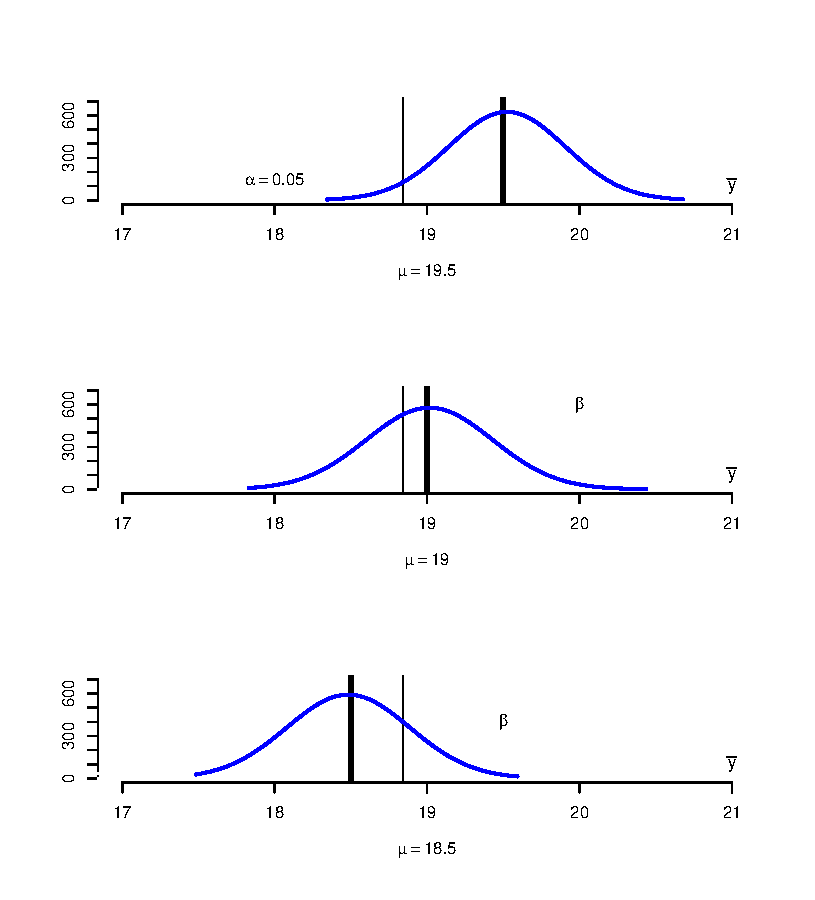
\includegraphics[width=0.8\linewidth]{Ch2_beta_dist.eps}
  \centering
  \caption{Effect of $\mu$ (mean) on $\beta$ (Type II error)}
  \label{fig:ch2_beta_dist}
\end{figure}
\
\begin{lstlisting}[language=R]
# Effect of mean on the Type II error
par(mfrow=c(3,1)) ; 
n = 300
x1 <- rnorm(n,mean = 19.5, sd=0.4)
h1 <- hist(x1,breaks = 1, xlim = c(17,21),ylim=c(0,700),
           border = "white",main="",xlab = expression(mu == 19.5),ylab = "") 
x1fit <- seq(min(x1),max(x1),length=length(x1)) ; abline(v=19.5,lwd=3) ; abline(v=18.842)
y1fit <- dnorm(x1fit,mean=mean(x1),sd=sd(x1)) ; y1fit <- y1fit*diff(h1$mids[1:2])*n
lines(x1fit,y1fit,col="blue", lwd=2)
text(18,150,expression(alpha == 0.05)) ; text(21,100,expression(bar(y)))

x2 <- rnorm(n,mean = 19, sd=0.4)
h2 <- hist(x2,breaks = 1, xlim = c(17,21),ylim=c(0,700),
           border = "white",main="",xlab = expression(mu == 19.0),ylab = "") 
x2fit <- seq(min(x2),max(x2),length=length(x2)) ; abline(v=19.0,lwd=3) ; abline(v=18.842)
y2fit <- dnorm(x2fit,mean=mean(x2),sd=sd(x2)) ; y2fit <- y2fit*diff(h2$mids[1:2])*n
lines(x2fit,y2fit,col="blue", lwd=2)
text(20,600,expression(beta)) ; text(21,100,expression(bar(y)))

x3 <- rnorm(n,mean = 18.5, sd=0.4)
h3 <- hist(x3,breaks = 1, xlim = c(17,21),ylim=c(0,700),
           border = "white",main="",xlab = expression(mu == 18.5),ylab = "") 
x3fit <- seq(min(x3),max(x3),length=length(x3)) ; abline(v=18.5,lwd=3) ; abline(v=18.842)
y3fit <- dnorm(x3fit,mean=mean(x3),sd=sd(x3)) ; y3fit <- y3fit*diff(h3$mids[1:2])*n
lines(x3fit,y3fit,col="blue", lwd=2)
text(19.5,400,expression(beta)) ; text(21,100,expression(bar(y)))
\end{lstlisting}
\
% EXAMPLES
\begin{equation}
\alpha
\end{equation}

\begin{figure}
  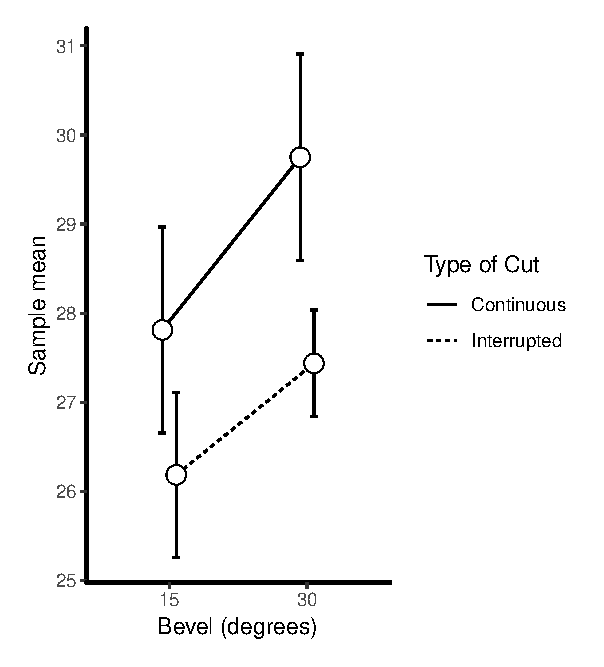
\includegraphics[width=0.2\linewidth]{Ch1_interaction_plot.eps}
  \centering
  \caption{$B \times C$ interaction for power requirement example}
  \label{fig:ch1_interaction}
\end{figure}

\begin{lstlisting}[language=R]
hello<-"hola"
\end{lstlisting}

\chapter[Single-Factor Experiment]{}

\begin{lstlisting}[language=R]
saludo <- 'hola'
\end{lstlisting}


\bibliographystyle{plain}
\bibliography{stats}


%%%%%%%%%%%%%%%%%%%%%%%%%%%%%%%%%%%%%%%%%%%%%%%%%%%%%%
%% optional prologue or prologues
% \chapter{Chapter Title}
% \prologue{<text>}{<author attribution>}

%%%%%%%%%%%%%%%%%%%%%%%%%%%%%%%%%%%%%%%%%%%%%
% Edited Book: Author and Affiliation
%%%%%%%%%%%%%%%%%%%%%%%%%%%%%%%%%%%%%%%%%%%%%

% After \chapter{Chapter Title}, you can
% enter the author name and embed the affiliation with
% \chapterauthors{(author name, or names)
% \chapteraffil{(affiliation or affiliations)}
% }    

% For instance:
% \chapter{Chapter Title}
% \chapterauthors{G. Alvarez and R. K. Watts
% \chapteraffil{Carnegie Mellon University, Pittsburgh, Pennsylvania}

% For separate affiliations you can use \affilmark{(number)} after
% the name of a particular author and before the matching affiliation:

% For instance:
% \chapter{Chapter Title}
% \chapterauthors{George Smeal, Ph.D.\affilmark{1}, Sally Smith,
% M.D.\affilmark{2}, and Stanley Kubrick\affilmark{1}
% \chapteraffil{\affilmark{1}AT\&T Bell Laboratories
% Murray Hill, New Jersey\\
% \affilmark{2}Harvard Medical School,
% Boston, Massachusetts}
% }

%%%%%%%%%%%%%%%%%%%%%%%

%% short version of section head, or one without \\ supplied in sq. brackets.

% \section[Introduction and fugue]{Introduction\\ and fugue}
% \subsection[This is the subsection]{This is the\\ subsection}
% \subsubsection{This is the subsubsection}
% \paragraph{This is the paragraph}

% \begin{chapreferences}{widest label}
% \bibitem{<label>}Reference
% \end{chapreferences}

% optional chapter bibliography using BibTeX,
% must also have \usepackage{chapterbib} before \begin{document}
% Must use root file with \include{chap1}, \include{chap2} form.
%\bibliographystyle{plain}
%\bibliography{<your .bib file name>}

% optional appendix at the end of a chapter:
% \chapappendix{<chap appendix title>}
% \chapappendix{} % no title

%%%%%%%%%%%%%%%%%%%%%%%%%%%%%%%%%%%%%%%%%%%%%%%%%%%%%%%%%%%%%%%%
%% End Matter >>>>>>>>>>>>>>>>>>

% \appendix{<optional title for appendix at end of book>}
% \appendix{} % appendix without title

% \begin{references}{<widest label>}
% \bibitem{sampref}Here is reference.
% \end{references}

%%%%%%%%%%%%%%%%%%%%%%%%%%%%%%%%%%%%%%%%%%%%%%%%%%%%%%%%%%%%%%%%
%% Optional Problem Sets: Can use this at the end of each chapter or at end
%% of book

% \begin{problems}
% \prob
% text

% \prob
% text

% \subprob
% text

% \subprob
% text

% \prob
% text
% \end{problems}

%%%%%%%%%%%%%%%%%%%%%%%%%%%%%%%%%%%%%%%%%%%%%%%%%%%%%%%%%%%%%%%%
%% Optional Exercises: Can use this at the end of each chapter or at end
%% of book

% \begin{exercises}
% \exer
% text

% \exer
% text

% \subexer
% text

% \subexer
% text

% \exer
% text
% \end{exercises}


%%%%%%%%%%%%%%%%%%%%%%%%%%%%%%%%%%%%%%%%%%%%%%%%%%%%%%%%%%%%%%%%
%% INDEX: Use only one index command set:

%% 1) The default LaTeX Index
\printindex

%% 2) For Topic index and Author index:

% \usepackage{multind}
% \makeindex{topic}
% \makeindex{authors}
% \begin{document}
% ...
% add index terms to your book, ie,
% \index{topic}{A term to go to the topic index}
% \index{authors}{Put this author in the author index}

%% (these are Wiley commands)
%\multiprintindex{topic}{Topic index}
%\multiprintindex{authors}{Author index}

\end{document}

%%%%%%% Demo of section head containing sample macro:
%% To get a macro to expand correctly in a section head, with upper and
%% lower case math, put the definition and set the box 
%% before \begin{document}, so that when it appears in the 
%% table of contents it will also work:

\newcommand{\VT}[1]{\ensuremath{{V_{T#1}}}}

%% use a box to expand the macro before we put it into the section head:

\newbox\sectsavebox
\setbox\sectsavebox=\hbox{\boldmath\VT{xyz}}

%%%%%%%%%%%%%%%%% End Demo


Other commands, and notes on usage:

-----
Possible section head levels:
\section{Introduction}
\subsection{This is subsection}
\paragraph{This is the paragraph}
\subsubsection{This is subsubsection}
\paragraph{This is the paragraph}

-----
Tables:
 Remember to use \centering for a small table and to start the table
 with \hline, use \hline underneath the column headers and at the end of 
 the table, i.e.,

\begin{table}[h]
\caption{Small Table}
\centering
\begin{tabular}{ccc}
\hline
one&two&three\\
\hline
C&D&E\\
\hline
\end{tabular}
\end{table}

For a table that expands to the width of the page, write

\begin{table}
\begin{tabular*}{\textwidth}{@{\extracolsep{\fill}}lcc}
\hline
....
\end{tabular*}
%% Sample table notes:
\begin{tablenotes}
$^a$Refs.~19 and 20.

$^b\kappa, \lambda>1$.
\end{tablenotes}
\end{table}

-----
Algorithm.
Maintains same fonts as text (as opposed to verbatim which uses fixed
width fonts). Space at beginning of line will be maintained if you
use \ at beginning of line.

\begin{algorithm}
{\bf state\_transition algorithm} $\{$
\        for each neuron $j\in\{0,1,\ldots,M-1\}$
\        $\{$   
\            calculate the weighted sum $S_j$ using Eq. (6);
\            if ($S_j>t_j$)
\                    $\{$turn ON neuron; $Y_1=+1\}$   
\            else if ($S_j<t_j$)
\                    $\{$turn OFF neuron; $Y_1=-1\}$   
\            else
\                    $\{$no change in neuron state; $y_j$ remains %
unchanged;$\}$ .
\        $\}$   
$\}$   
\end{algorithm}

-----
Sample quote:
\begin{quote}
quotation...
\end{quote}

-----
Listing samples

\begin{enumerate}
\item
This is the first item in the numbered list.

\item
This is the second item in the numbered list.
\end{enumerate}

\begin{itemize}
\item
This is the first item in the itemized list.

\item
This is the first item in the itemized list.
This is the first item in the itemized list.
This is the first item in the itemized list.
\end{itemize}

\begin{itemize}
\item[]
This is the first item in the itemized list.

\item[]
This is the first item in the itemized list.
This is the first item in the itemized list.
This is the first item in the itemized list.
\end{itemize}

%% Index commands
Author and Topic Indices, See docs.pdf and w-bksamp.pdf
